\chapter{Introduction}

\section{Structure and Content}
\begin{itemize}

    \item \textbf{Module 1}: 
    \begin{enumerate}
        \item \textbf{\textit{intra-vehicles communications}}: nodes, sensors, ECU
        \item \textbf{\textit{signal busses}}: CAN, LIN, FlexRay, MOST, Ethernet [ T1/T1S]
        \item \textbf{\textit{car domain and OS}}
    \end{enumerate}
    
    \item \textbf{Module 2}:
    \begin{enumerate}
        \item \textbf{\textit{inter-vehicles communications}}: \textit{V2V} and \textit{V2X} (car is a node)
        \item \textbf{\textit{wireless technologies}}: Bluetooth, LoRa, C-V2X, IEE 802.11p (bd)
        \item application, messages, broadcast, GPS
    \end{enumerate}

\end{itemize}
Different \textbf{domain} or \textbf{application} needs different \textit{communications protocols}, is important to understand how each nodes in domain communicate each other (inside the car).

\newpage
\section{Intra-Vehicles}
From the 80's, where the car's control unit are isolated an there was a dedicated wires connect sensors and actuators with less electronic than now, until the reach the greatest goal of evolution in the automotive sector: autonomous drive. The complexity of the number of connection from each ECU's to the other, also the number of ECU's for each car, is growing. While the number of signal increase in a liner way, the connection between ECU's is growing with a quadratic complexity $O(n^2)$.

If we examine the evolutions of the ECUs number inside an ``Audi A6'' we can observe that in 1997 it has 5 ECUs and in the 2007 it has 50 ECUs, instead the ``Tesla M3'' in the 2017 has 70 ECUs. The quadratic increase of ECUs number, however has reach a cap for two main reason: the cost and the space inside the car. Traditionally one ECUs is responsible of one task, but nowadays it could be two type of trends:
\begin{enumerate}[nosep]
    \item \textit{distributed of function across ECUs}
    \item \textit{integration of multiple function in one ECU}
\end{enumerate}

\section{Architectures}

\begin{figure}[h]
    \centering
    \begin{minipage}[t]{0.45\textwidth}
        \centering
        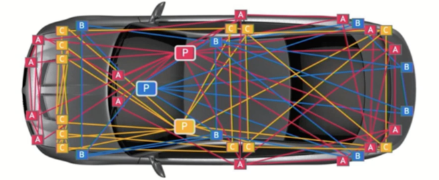
\includegraphics[width=\textwidth]{img/domain_architecture}
        \caption{\textit{Domain Architecture}}
        
        \begin{flushleft}
            \begin{enumerate}[nosep]
                \item central domain controller (\textbf{P}) or high performance computer
                \item ability to handle more complex functions
                \item cost optimization
                \item cable harness is rigid and expensive
            \end{enumerate}
        \end{flushleft}

    \end{minipage}
    \begin{minipage}[t]{0.45\textwidth}
        \centering
        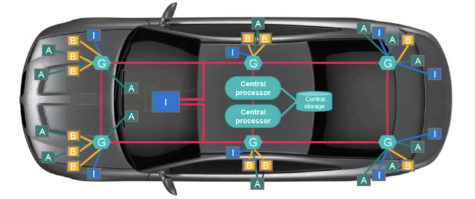
\includegraphics[width=\textwidth]{img/zonal_architecture}
        \caption{\textit{Zonal Architecture}}
        
        \begin{flushleft}
            \begin{enumerate}[nosep]
                \item local ethernet per zone (\textbf{G})
                \item ultra high-speed secured backbone between zone
                \item centralized software
                \item central computer storage
            \end{enumerate}
        \end{flushleft}
        
    \end{minipage}
\end{figure}

\section{Basic Knowledge}

\subsection{Multiple Access Protocols}
In the ISO/OSI stack the first layer is the \textit{data link layer} and it is used, in a computer network, to transmit the data between two or more devices or nodes. The data link layer it is normally split in two different sub-layer:
\begin{enumerate}[nosep]
    \item \textbf{data link control}: is a reliable channel for transmitting data over a dedicated link using various techniques such as framing, error control and flow control of data packets in the computer network.
    \item \textbf{multiple access protocol}: if the link doesn't connect only two nodes, but multiple nodes can access to the physical link is possible that two or more nodes start to communicate in the same time, and it could be possible to have collision and cross talk between two or more devices. In this case the \textit{multiple access protocol} is required to reduce the collision and avoid cross talk between the channel.
\end{enumerate}

\resizebox{\textwidth}{!}{%
\begin{forest}
  for tree={
    child anchor=west,
    parent anchor=east,
    grow'=east,
    text width=4cm,
    draw,
    anchor=west,
    edge path={
      \noexpand\path[\forestoption{edge}]
        (.child anchor) -| +(-5pt,0) -- +(-5pt,0) |-
        (!u.parent anchor)\forestoption{edge label};
    },
  }
    [\textbf{\textit{Multiple Access protocols}}
        [\textbf{Channelization Protocols}
            [\textit{FDMA}
                [frequency division multiple access]
            ]
            [\textit{TDMA}
                [time division multiple access]
            ]
            [\textit{CDMA}
                [code division multiple access]
            ]
        ]
        [\textbf{Control Access Protocols}: a single station cannot send frame if all the other don't approved 
            [\textit{Reservation}]
            [\textit{Polling}]
            [\textit{Token Passing}]
        ]
        [\textbf{Random Access Protocols}
            [\textit{ALOHA}: it is design for wireless LAN
                [\textbf{Pure ALOHA}]
                [\textbf{Slotted ALOHA}]
            ]
            [\textit{CSMA}
                [1-Persistent]
                [Non-Persistent]
                [P-Persistent]
                [O-Persistent]
            ]
            [\textit{CSMA/CD}]
            [\textit{CSMA/CA}]
        ]
    ]
\end{forest}
}

In this course it could be useful to see in dept three type of \textit{Multiple Access Protocols}: the first one is \textbf{\textit{Carrier Sense Multiple Access - Collision Detection}}, next is the \textbf{\textit{Carrier Sense Multiple Access - Collision Avoidance}} and the last one is the \textbf{\textit{Time Division Multiple Access}}. In the autonomotive domain indeed there is needs to have a bus topology network and it is important to avoid collision. \\ \newline
\textbf{\textit{CSMA/CA - Carrier Sense Multiple Access - Collision Avoidance}}: the idea is that before transmitting, a node first listens the shared medium to determine if the channel is not used (\textbf{idle}), if not it could start to transmit, but the problem start when two nodes begins to write on the nodes together. The \textbf{Collision Avoidance} part get in the game when two or more device try to write in the channel simultaneously in this case if another nodes is sense the transmitting node wait for a period of time (usually random) before re-start the writing procedure. \\ \newline
\textbf{\textit{CSMA/CD - Carrier Sense Multiple Access - Collision Detection}}: is use in early Ethernet technology for LAN. It use carrier-sense to detect if the media is \textbf{idle} and it is combined with collision-detection in which a transmission station sense collision by detecting transmissions from other stations while it is transmitting a frame.
\begin{enumerate}[nosep]
    \item is the frame ready for the transmission? if not, wait for the frame.
    \item is medium idle? if not, wait until it becomes ready.
    \item start transmission and monitor for collision during transmission.
    \item did a collision occur? if yes, go to collision detecting procedure.
    \begin{enumerate}[nosep]
        \item continue the transmission (with \textbf{jam signal}) until minimum packet time is reached to ensure that all receiver detect the collision.
        \item increment re-transmission counter.
        \item was the maximum number of transmission (time out) attempts reached? if yes, abort transmission.
        \item restart from 1.
    \end{enumerate}
    \item reset the transmission counter and complete frame transmission.
\end{enumerate}

\textbf{\textit{TDMA - Time Division Multiple Access}}: is a channel access method for share-medium networks. It allow several users to share the same \textit{frequency channel} by dividing the signal into different time slot. The users transmit in rapid succession, one after the other, each using its own time slot. This type of access to the physical medium has higher syncronization overhead tha \textit{CSMA}.

\subsection{Bit Coding}
The first thing is to introduce the \textbf{\textit{Electromagnetic Inferference - EMI}} that is a disturbance generate by an external source that affects an electrical circuit by \textit{electromagnetic induction}, \textit{electromagnetic couplig} or from conduction. For reduce EMI there are three possible way: add shield to wires, used twisted pair wiring or use coding with few rising/falling signal edges. At this point we can introduce the two main coding techniques: \textbf{\textit{NRZ - Non Return to Zero}} or \textbf{\textit{Manchester Coding}} (original variant).
\begin{figure}[h]
    \centering
    \begin{minipage}[t]{0.45\textwidth}
        \centering
        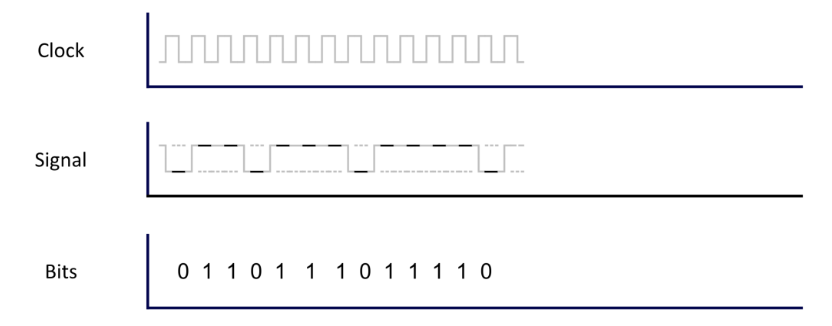
\includegraphics[width=\textwidth]{img/nrz_coding}
        \caption{\textit{Non Return to Zeros}}
        
        \begin{flushleft}
            In the \textbf{\textit{Non Return to Zero}} the digital ones is, usually, the positive voltage, while digital zeros are represented by other significat condition, like negative voltage.
        \end{flushleft}

    \end{minipage}
    \begin{minipage}[t]{0.45\textwidth}
        \centering
        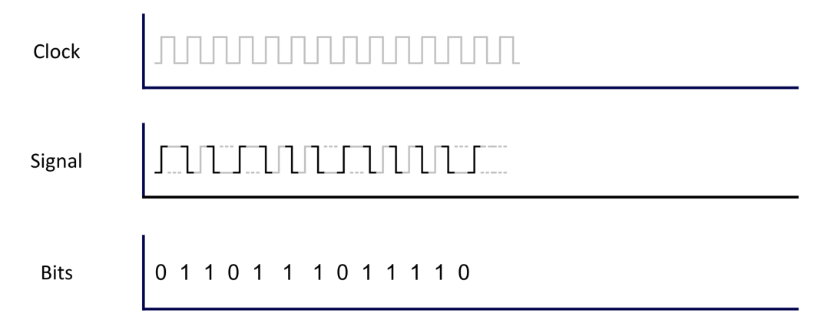
\includegraphics[width=\textwidth]{img/m_coding}
        \caption{\textit{Manchester Coding}}
        
        \begin{flushleft}
            In the \textbf{\textit{Manchester Coding}} (original variant) the digital ones is the rising edge of the signal, instead the digital zeros are represented by the falling edge of the signal.
        \end{flushleft}
        
    \end{minipage}
\end{figure}

In both case it must be identify the digital zeros or one on the rising edge of the clock, so the syncronization problem between the clock of the transmitting node and the receiving nodes it is foundamentals.